\documentclass[11pt,a4paper]{article}
\usepackage[utf8]{inputenc}
\usepackage{graphicx}
\usepackage{url}
\usepackage{xspace}
\usepackage{amsmath}
\usepackage{hyperref}
\usepackage[usenames,dvipsnames]{color}
\usepackage{listings}
\newcommand{\CodeSymbol}[1]{\textcolor{Bittersweet}{#1}}
\lstset{
   language=Ada,
   keywordstyle=\color{RedViolet}\ttfamily\bf,
   showspaces=false,
   basicstyle={\scriptsize \sffamily},
   commentstyle=\color{red}\textit,
   stringstyle=\color{MidnightBlue}\ttfamily,
   showtabs=false,
   showstringspaces=false,
   morekeywords=[1]Pre,
   morekeywords=[1]Post,
   morekeywords=[1]Test\_Case,
   morekeywords=[1]Contract\_Cases,
   morekeywords=[1]some,
   morekeywords=[1]Old,
   morekeywords=[1]Global,
   morekeywords=[1]Depends,
   morekeywords=[1]Loop\_Invariant,
   morekeywords=[1]Loop\_Variant,
   morekeywords=[1]Loop\_Entry,
   morekeywords=[1]Increases,
   literate={(}{{\CodeSymbol{(}}}1
            {)}{{\CodeSymbol{)}}}1
            {>}{{\CodeSymbol{$>$}}}1
            {>=}{{\CodeSymbol{$\ge$}}}1
            {<}{{\CodeSymbol{$<$}}}1
            {<=}{{\CodeSymbol{$\le$}}}1
            {=}{{\CodeSymbol{$=$}}}1
            {:}{{\CodeSymbol{$:$}}}1
            {.}{{\CodeSymbol{$.$}}}1
            {;}{{\CodeSymbol{$;$}}}1
            {/=}{{\CodeSymbol{$\ne$}}}1
            {=>}{{\CodeSymbol{$\Rightarrow$}}}1
            {->}{{\CodeSymbol{$\rightarrow$}}}1
            {<->}{{\CodeSymbol{$\leftrightarrow$}}}1
}

\newcommand{\DO}{\textsc{do-178}\xspace}
\newcommand{\DOB}{\textsc{do-178b}\xspace}
\newcommand{\DOC}{\textsc{do-178c}\xspace}
\newcommand{\hilite}{Hi-Lite\xspace}
\newcommand{\openetcs}{openETCS\xspace}
\newcommand{\gnatprove}{GNATprove\xspace}
\newcommand{\oldspark}{SPARK~2005\xspace}
\newcommand{\newspark}{SPARK~2014\xspace}
\newcommand{\spark}{SPARK\xspace}
\newcommand{\ada}{Ada\xspace}
\newcommand{\adatwtw}{Ada~2012\xspace}
\newcommand{\altergo}{Alt-Ergo\xspace}

\newcommand{\etc}{\textit{etc.}\xspace}
\newcommand{\ie}{\textit{i.e.}\xspace}
\newcommand{\adhoc}{\textit{ad hoc}\xspace}
\newcommand{\Eg}{\textit{E.g.}\xspace}
\newcommand{\eg}{\textit{e.g.}\xspace}
\newcommand{\etal}{\textit{et al.}\xspace}
\newcommand{\wrt}{w.r.t.\xspace}
\newcommand{\aka}{a.k.a.\xspace}
\newcommand{\resp}{resp.\xspace}

\urlstyle{sf}

\begin{document}

\title{Auto-Active Proof of Red-Black Trees in SPARK}

\author{%
\large Claire Dross and Yannick Moy\\
\normalsize AdaCore, 46 rue d'Amsterdam, F-75009 Paris (France)}

\date{}

\maketitle

\paragraph{Abstract}
SPARK is a subset of the Ada programming language targeted at safety- and
security-critical applications. SPARK formal verification toolset allows to
guarantee that a SPARK program is free from broad classes of errors (like reads
of uninitialized data and run-time errors) and that it complies with its
specification. While the former is a well adopted practice among SPARK users,
the latter is used much more narrowly, owing to the cost of specifying the
behavior of programs and even more the cost of achieving proof of such
specifications. SPARK relies on automatic provers to keep the cost of formal
verification reasonable, and on the techniques of auto-active verification for
interacting with automatic provers. In this paper, we present how we applied
auto-active verification to formally verify a library of red-black trees. To
the best of our knowledge, this is the most advanced use of auto-active
verification so far.

\paragraph{Keywords}
System formal development, Verification and validation,
Certification and dependability

\section{Introduction}

\section{Preliminaries}
\subsection{SPARK 2014}
\subsection{Auto-active Verification}
\subsection{Red-Black Trees}

\section{Red-Black Trees in SPARK}
\subsection{Invariants and Models}
% invariants of data structures
% relation between invariants and models
% public model of RBT
% internal model of tree

% hierarchy done with proof in mind, separation of concerns
%    binary_trees => tree structure
%    search_trees => ordered values
%    red_black_trees => balanceness
% properties stored in (private) invariants and reflected in (public) models
%    binary_trees => reachability
%    search_trees => set of contained values
%    red_black_trees => no model
% models should be easy to use/complex to verify to factor complexity
%  ex: provide a model of reachability
% primitives needed by upper levels provided at lower level were they abide by the invariant

Though they are relatively complex data structures, implementing red black trees
correctly is not a challenge as numerous implementations and descriptions of the
algorithm are readily available.
However, it is generally agreed that, to achieve
full static verification of a complex algorithm, it is better to design the
software from the start with proof in mind (cite?).
To this aim, we have divided our implementation of red black trees in three
distinct parts, each concerned only in part of the data structure properties.

The first part defines binary trees. It is only concerned with properties
relative to the tree structure of the underlying memory.
The second part associates values to nodes of binary trees to define search trees.
It is concerned with order of values in the tree.
The third part enforces balancedness using the classical red black tree coloring
mechanism.

At each level, the separation of concerns is ensured by the use of type invariants.
As defined by Ada 2012 standard, type invariants are boolan properties associated
to private types which can be temporarily violated in the private functions of the
type but must always hold outside of the type's private scope.
More precisely, the property that should be ensured at each level (tree structure,
order of values, or balancedness) is enforced at the boundary of every function
of this level and then assumed in upper levels.

As an example, let us look at the invariant of binary trees. Binary trees are
encoded using an imperative datastructure as represented in Figure~\ref{fig-binary}.
Each node contains a reference to is right and left child if any as well as a
reference to its parent and a position, which may be Top, for the root, or
Right or Left depending on their position with respect to their parent.

\begin{figure}[ht]
\begin{center}
\includegraphics[width=4cm]{tree_structure.pdf}
\includegraphics[width=5cm]{binary_1.pdf}
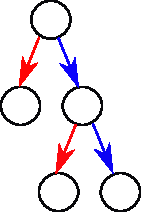
\includegraphics[width=2cm]{binary_2.pdf}
\caption{\label{fig-binary} From left to right: Representation of nodes in binary trees.
Example of a binary tree, for readability, parents and positions are not represented.
The binary tree represented in previous figure.}
\end{center}
\end{figure}

The invariant of binary trees is given in Figure~\ref{fig-binary-inv}.
As can be seen, it is only concerned with low level sanity of the
tree representation.

\begin{figure}[ht]
\begin{lstlisting}
 --  Cells that are not allocated yet have default values

(for all I in F.S + 1 .. Max => F.C (I) = (Empty, Empty, Empty, Top))

--  Parent and children of all cells are allocated or empty

and then (for all I in Index_Type => F.C (I).Parent in Empty .. F.S)
and then (for all I in Index_Type => F.C (I).Left in Empty .. F.S)
and then (for all I in Index_Type => F.C (I).Right in Empty .. F.S)

--  If a cell is the root of a tree (position Top) it has no parent

and then (for all I in Index_Type =>
           (if F.C (I).Position = Top then F.C (I).Parent = Empty))

--  If a cell I has a left child, then its left child has position
--  Left and parent I.

and then (for all I in Index_Type =>
           (if F.C (I).Left /= Empty then
              F.C (F.C (I).Left).Position = Left
              and then F.C (F.C (I).Left).Parent = I))

--  If a cell I has a right child, then its right child has position
--  Right and parent I.

and then (for all I in Index_Type =>
           (if F.C (I).Right /= Empty then
             F.C (F.C (I).Right).Position = Right
             and then F.C (F.C (I).Right).Parent = I))

--  If a cell is a child (position Left or Right), then it is the
--  child of its parent.

and then (for all I in Index_Type =>
           (if F.C (I).Parent /= Empty and then F.C (I).Position = Left
            then F.C (F.C (I).Parent).Left = I))
and then (for all I in Index_Type =>
           (if F.C (I).Parent /= Empty and then F.C (I).Position = Right
            then F.C (F.C (I).Parent).Right = I))
\end{lstlisting}
\caption{\label{fig-binary-inv} Type invariant of binary trees.}
\end{figure}

{\color{red} TODO: Rewrite using Parent (I) instead of F.C (I).Parent?
Remove reference to size or explain it?}

So that the properties deriving from lower levels is available to upper levels, we
introduce model functions. These functions rely on the private invariant of the type
to construct a high level view of the datastructure that can then be used to express
complex porperties over the structure.

As an example, reachability in the tree structure is a complex property, that is
crucial to reason about search trees. Reachability is difficult to tackle for SPARK
as it is an inductive porperty, and therefore requires inductive proofs. To factor out
this complexity at the binary tree level, we introduce
a model of binary trees allowing to reason easily about branches in the tree, see
Figure~\ref{fig-binary-mod}.

\begin{figure}[ht]
\begin{lstlisting}
type Position_Type is (Left, Right, Top);
subtype Direction is Position_Type range Left .. Right;

package D_Seq is new Conts.Functional.Sequences
  (Positive_Count_Type, Direction);
use D_Seq;
--  Sequence of directions modelling a path from the root of the tree
--  to a node in the tree.

type Path_Type is record
   A : Sequence;
   K : Boolean := False;
end record
with Predicate => Length (A) <= Max;
--  Type used to model the path from the root of a tree to a given node,
--  which may or not be in the tree:
--    - if a node is in the tree, the corresponding path will have K =
--      True, and A will denote the path from the root to this node.
--    - if a node is not in the tree, the corresponding path will have
--      K = False and A will be empty.
\end{lstlisting}
\caption{\label{fig-binary-mod} Model of branches in a binary tree.}
\end{figure}

The model of a binary tree associates a sequence of directions, namely
Right or Left, to each node in the binary tree. An additional boolean encodes
whether the is reachable from the root. Figure~\ref{fig-binary-mod-ex} gives
the model of the binary tree presented in Figure~\ref{fig-binary}.

\begin{figure}[ht]
\begin{center}
\includegraphics[width=5cm]{model.pdf}
\caption{\label{fig-binary-mod-ex} Example of model of a binary tree.}
\end{center}
\end{figure}

Only valid binary trees are associated a model, that is, the model function
only works on trees for which the tree structure invariant holds. As a result,
we cannot use this model function inside the implemenation of binary tree,
for example to state in the invariant that all the nodes are reachable from the
root (there is no memory leak). However, as type invariants always hold outside
of data structures implementation, the path model can safely be used on any
binary tree in the implementation of search trees. In particular, we use it
in the invariant of search trees, which is given in Figure~\ref{fig-search-inv}.

\begin{figure}[ht]
\begin{lstlisting}
(for all I in Index_Type =>
  (for all J in Index_Type =>
    (if Model (F, Root) (I).K
       and then Model (F, Root) (J).K
       and then Model (F, Root) (I).A < Model (F, Root) (J).A
     then (if Get (Model (F, Root) (J).A,
                   Length (Model (F, Root) (I).A) + 1) = Left
           then Values (J) < Values (I)
           else Values (J) > Values (I)))))
\end{lstlisting}
\caption{\label{fig-search-inv} Type invariant of search trees.}
\end{figure}

The invariant of search trees states that the value stored in each node of the
tree is bigger than all the values stored in the subtree rooted at its left
child and smaller than all the values stored in the subtree rooted at its right
child. An example of values that would fit the tree from Figure~\ref{fig-binary}
is given in Figure~\ref{fig-search}. To express this invariant, we use the 
model of the underlying binary tree. A value V is stored in the subtree rooted
at the right child of a node if the path leading to this value is a supersequence
of the path leading to V and the next element in the sequence is Right.

\begin{figure}[ht]
\begin{center}
\includegraphics[width=2cm]{search.pdf}
\caption{\label{fig-search} Ordered nodes in a search tree.}
\end{center}
\end{figure}

{\color{red} TODO: speak about red black trees}

\begin{figure}[ht]
\begin{center}
\includegraphics[width=2cm]{red_black.pdf}
\end{center}
\end{figure}

\subsection{Proof Principles}
% principle of inductive proofs on size of path
% principles of dealing with the frame condition: unmodified trees in forest

% reachability requires proof by induction on the size of the path
%   This is done using loops and loop invariants
% order requires case split
%   This is done using if statements
\subsection{Ghost Code}
% different uses of ghost code

% For specification purpose:
% - typically ghost functions used in contracts
% - can be interesting to execute as test oracles
% For verification purpose:
% - typically ghost procedures containing proofs by induction (loops), by case analysis...
% - no need to execute them, they do not bring anything
% No way to distinguish between both right now.
\subsection{Implementation}
% no pointer in spark => indexes inside an array
% avoid copies, use forest
% it is bounded
% values and colors are outside, in separate array (to avoid having them in the frame)
% provide plug/extract to modify the forest while keepong the invariant
% rotate_left and rotate_right preserve the order
\subsection{Specification}
% use parent/position and model
% model can be derived from parent and position but have it in post to do inductive proofs only once
\subsection{Auto-active Verification}
% factored out in ghost procedures to keep efficiency
% with or without contracts (inlining)

\section{Development and Verification Data}
% number of assertions, loc of ghost code, etc.
% data on automatic verification
% feedback from development and verification cycles

\section{Related Work}

\section{Conclusion}


\paragraph*{Acknowledgements}


\bibliographystyle{plain}
\bibliography{nfm_2017}

\end{document}
